\chapter{Results}
%Results:
%	-Total active days pre+post-trimming
%	-Total count of sp events (also pre+post?)
%-Overall detection rate pattern in all species
%-Overall activity pattern in all species
%(-Density curves throughout the year, obs per (week/month)) %Don't think so
%-Intro to how each sp will be presented


The type of CT flash had an overall minor effect on detection rates.
In general, the control periods (which never had white flashes) had a somewhat lower detection rate than the IR and white LED periods.
%Between the experiment periods, I expected the IR periods to have the highest detection rate, but LED was somewhat higher for most species (see table \ref{tab:params}). %AMkomm: why?

There were a total of $\approx 18 000$ camera trapping days, which was unevenly distributed between the different periods and period types.

%Trimming the data according to median period length of IR periods (which was shorter than that of control and white LED periods) evened out the disproportions between the periods (see figure \ref{fig:active days}). %IMRkomm: Dette har du allerede sagt i metode



I will present detailed results of all the nine mammalian species included in my analyses, grouped by taxonomic order and family, in order from most to least number of events, as shown in figure \ref{fig:events}.
Each species is presented with a figure showing activity across time of day, a photo taken with a white LED CT of the species, %TODO (during night) 
an equivalence test, and a plot of the marginal means of the fixed effects in the GLMM model, showing the detection rates of all three types of periods (Control, IR and white LED) along a time axis.


\begin{figure}[h]
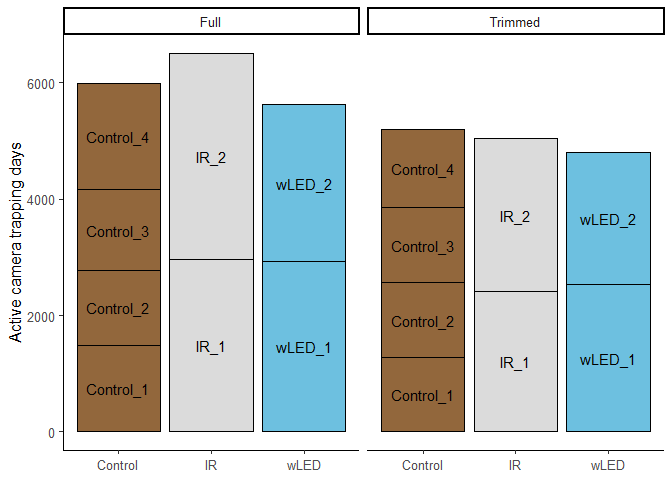
\includegraphics[width=0.9\linewidth]{../R/glmm_sp_files/figure-html/active-days-3.png} 
	\caption{Active camera days per periods}
	\label{fig:active days}
\end{figure}


\begin{figure}[h]
 \centering
	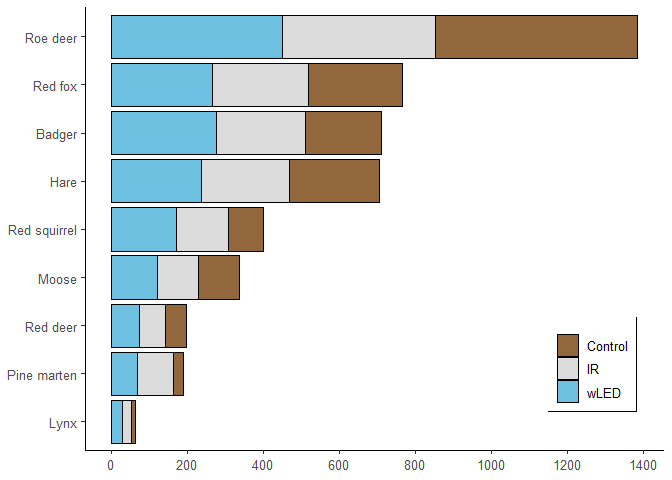
\includegraphics[scale=.4]{../R/glmm_sp_files/figure-html/events-1.png}
 \caption[Raw count and number of events per species]
 {Raw count and number of events per species}
\caption{Camera trapping days and number of events per species}
\label{fig:events}
\end{figure}


The main effect of LED was positive for most species, although none responded significantly (table \ref{tab:param}). % IMRkomm: Det er vanskelig å si noe generelt om en main effect når denne også er med i (signifikante) interaksjoner. Og all den tid denne heller ikke er signifikant, så trenger du ikke nevne hvilken retning den tar. Dette er også en kategorisk variabel, så dette estimatet gir forskjellen fra referansenivået (her: kontroll), ikke en global effekt. Og denne effekten er igjen påvirket av interaksjonene den deltar i.
\clearpage

\begin{table}[ht]  % må inn for å fjerna begin{table} kvar gong tabellen oppdaterast!

\caption[Model results]
{ \footnotesize 
Results of Poisson mixed effects models on detection rate of species at 56 different locations in southeastern Norway, with three different treatment levels interacting with time since deployment (Time); periods from sites unchanged through the the whole study period (Intercept), periods with only IR camera (IR), periods with an additional white LED camera (wLED). Random effects are location ID and week of year. %TODO random effects st.dev.
%95\% Confidence Intervals and p-values were computed using the Wald approximation.
}
\label{tab:param}
\footnotesize
% latex table generated in R 4.0.4 by xtable 1.8-4 package
% Fri Mar 26 20:35:32 2021
\centering
{\tiny\renewcommand{\arraystretch}{.8}
	\resizebox{!}{.35\paperheight}{%
		\begin{tabular}[c]{llrlcrrr}
  \toprule
Species & Parameter & Coefficient & SE & 95\% CI & z & p & SGPV \\ 
\midrule
Roe deer & Intercept & -2.85 & 0.38 & (-3.58, -2.11) & -7.57 & $<$ .001 & 0.00 \\ 
& Time & -0.05 & 0.02 & (-0.09, -0.01) & -2.24 & \textbf{0.025}  & \textit{1.00} \\ 
& IR & -0.26 & 0.44 & (-1.12,  0.60) & -0.59 & 0.557  & 0.14 \\ 
& wLED & -0.13 & 0.44 & (-0.99,  0.73) & -0.30 & 0.761  & 0.14 \\ 
& Time * IR & 0.02 & 0.03 & (-0.04,  0.08) & 0.71 & 0.476  & \textit{1.00} \\ 
& Time * wLED & $<$ 0.01 & 0.03 & (-0.05,  0.06) & 0.12 & 0.901  & \textit{1.00} \\ 
\midrule
Moose & Intercept & -4.15 & 0.30 & (-4.75, -3.56) & -13.75 & $<$ .001 & 0.00 \\ 
& Time & $<$ 0.01 & 0.05 & (-0.08,  0.10) & 0.14 & 0.890  & \textit{1.00} \\ 
& IR & 		-0.08 & 0.35 & (-0.77,  0.60) & -0.23 & 0.814  & 0.17 \\ 
& wLED & 	 0.30 & 0.34 & (-0.36,  0.97) & 0.89 & 0.373  & 0.18 \\ 
& Time * IR & 0.05 & 0.06 & (-0.06,  0.17) & 0.86 & 0.389  & 0.75 \\ 
& Time * wLED & $<$ 0.01 & 0.06 & (-0.12,  0.10) & -0.12 & 0.902  & \textit{1.00} \\ 
\midrule
Red deer & Intercept & -3.89 & 0.41 & (-4.69, -3.09) & -9.55 & $<$ .001 & 0.00 \\ 
& Time & -0.09 & 0.06 & (-0.21,  0.02) & -1.63 & 0.104  & 0.53 \\ 
& IR & $<$ 0.01 & 0.50 & (-0.99,  0.97) & -0.02 & 0.984  & 0.12 \\ 
& wLED & -0.69 & 0.53 & (-1.72,  0.35) & -1.30 & 0.192  & 0.12 \\ 
& Time * IR & 0.06 & 0.08 & (-0.09,  0.21) & 0.81 & 0.421  & 0.65 \\ 
& Time * wLED & 0.23 & 0.08 & ( 0.08,  0.38) & 2.96 & \textbf{0.003}  & 0.00 \\ 
\midrule
Badger & Intercept & -4.49 & 0.37 & (-5.22, -3.76) & -12.12 & $<$ .001 & 0.00 \\ 
& Time & 0.06 & 0.03 & ( 0.00,  0.13) & 1.85 & 0.064  & 0.82 \\ 
& IR & 0.17 & 0.39 & (-0.59,  0.93) & 0.44 & 0.657  & 0.16 \\ 
& wLED & 0.24 & 0.38 & (-0.51,  0.99) & 0.64 & 0.523  & 0.16 \\ 
& Time * IR & 0.01 & 0.04 & (-0.07,  0.09) & 0.27 & 0.784  & \textit{1.00} \\ 
& Time * wLED & $<$ 0.01 & 0.04 & (-0.07,  0.08) & 0.11 & 0.914  & \textit{1.00} \\ 
\midrule
Pine Marten & Intercept & -5.95 & 0.54 & (-7.02, -4.89) & -10.95 & $<$ .001 & 0.00 \\ 
& Time & 0.09 & 0.09 & (-0.09,  0.28) & 0.97 & 0.331  & 0.52 \\ 
& IR & 1.69 & 0.58 & ( 0.55,  2.82) & 2.92 & \textbf{0.004}  & 0.00 \\ 
& wLED & 0.76 & 0.61 & (-0.43,  1.95) & 1.25 & 0.210  & 0.10 \\ 
& Time * IR & -0.11 & 0.11 & (-0.32,  0.09) & -1.07 & 0.286  & 0.46 \\ 
& Time * wLED & 0.03 & 0.11 & (-0.18,  0.24) & 0.30 & 0.768  & 0.56 \\ 
\midrule
Red fox & Intercept & -3.44 & 0.26 & (-3.94, -2.94) & -13.40 & $<$ .001 & 0.00 \\ 
& Time & $<$ 0.01 & 0.03 & (-0.06,  0.05) & -0.02 & 0.985  & \textit{1.00} \\ 
& IR & 0.03 & 0.32 & (-0.59,  0.65) & 0.09 & 0.926  & 0.19 \\ 
& wLED & 0.18 & 0.31 & (-0.44,  0.79) & 0.56 & 0.574  & 0.19 \\ 
& Time * IR & $<$ 0.01 & 0.04 & (-0.08,  0.07) & -0.06 & 0.949  & \textit{1.00} \\ 
& Time * wLED & -0.01 & 0.04 & (-0.08,  0.06) & -0.30 & 0.763  & \textit{1.00} \\ 
\midrule
Lynx & Intercept & -4.82 & 0.58 & (-5.96, -3.67) & -8.24 & $<$ .001 & 0.00 \\ 
& Time & -0.22 & 0.14 & (-0.49,  0.05) & -1.58 & 0.113  & 0.24 \\ 
& IR & -0.20 & 0.72 & (-1.61,  1.21) & -0.28 & 0.781  & 0.08 \\ 
& wLED & 0.15 & 0.72 & (-1.26,  1.55) & 0.20 & 0.839  & 0.08 \\ 
& Time * IR & 0.25 & 0.16 & (-0.07,  0.57) & 1.53 & 0.127  & 0.22 \\ 
& Time * wLED & 0.26 & 0.16 & (-0.06,  0.58) & 1.59 & 0.112  & 0.20 \\ 
\midrule
Hare & Intercept & -3.91 & 0.36 & (-4.61, -3.21) & -10.94 & $<$ .001 & 0.00 \\ 
& Time & 0.04 & 0.03 & (-0.03,  0.10) & 1.12 & 0.263  & \textit{1.00} \\ 
& IR & 0.38 & 0.42 & (-0.44,  1.21) & 0.91 & 0.363  & 0.14 \\ 
& wLED & 0.25 & 0.42 & (-0.58,  1.08) & 0.59 & 0.555  & 0.14 \\ 
& Time * IR & -0.05 & 0.04 & (-0.13,  0.03) & -1.26 & 0.209  & 0.88 \\ 
& Time * wLED & $<$ 0.01 & 0.04 & (-0.08,  0.08) & 0.03 & 0.975  & \textit{1.00} \\ 
\midrule
Red squirrel & Intercept & -4.82 & 0.41 & (-5.63, -4.00) & -11.63 & $<$ .001 & 0.00 \\ 
& Time & 0.08 & 0.05 & (-0.01,  0.18) & 1.67 & 0.095  & 0.62 \\ 
& IR & 0.91 & 0.47 & (-0.02,  1.83) & 1.93 & 0.054  & 0.00 \\ 
& wLED & 0.61 & 0.48 & (-0.32,  1.54) & 1.28 & 0.201  & 0.13 \\ 
& Time * IR & -0.17 & 0.06 & (-0.29, -0.05) & -2.85 & \textbf{0.004}  & 0.13 \\ 
& Time * wLED & -0.02 & 0.06 & (-0.13,  0.10) & -0.29 & 0.771  & 0.92 \\ 
   \bottomrule
\end{tabular}}}

%IMRkomm:
%Ta bort parentes rundt «intercept», skriv i teksten at TimeDeploy = time since deployment of camera, kanskje også forklare hva IR og white LED er i teksten. Skriv at referansenivået for flash type er control. Fp med hvilke random effects du har brukt, og før opp stdev for disse. 
%Kanskje markere signifikante effekter med bold eller kursiv, for å lette lesingen?

\pagestyle{empty}
%

\begin{figure}
		\begin{subfigure}{.5\textwidth}
		  \centering
		  	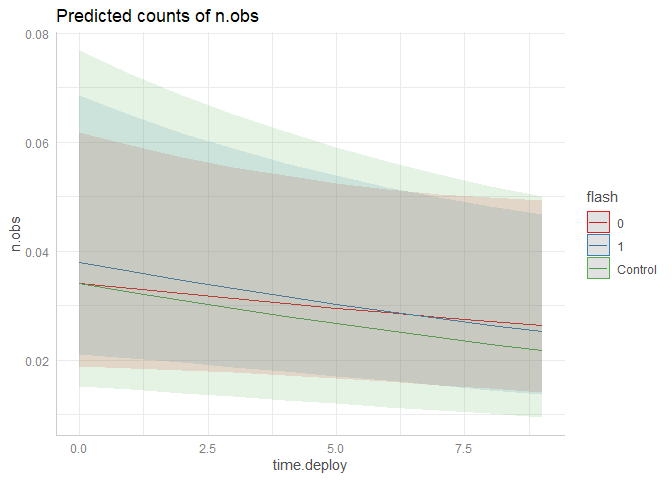
\includegraphics[width=.8\linewidth]{../R/glmm_sp_files/figure-gfm/raadyr-C-report-1.png}
		  \caption{Roe deer}
		  	\label{fig:glmm_raa}
	\end{subfigure}
		\begin{subfigure}{.5\textwidth}
		  \centering
		  	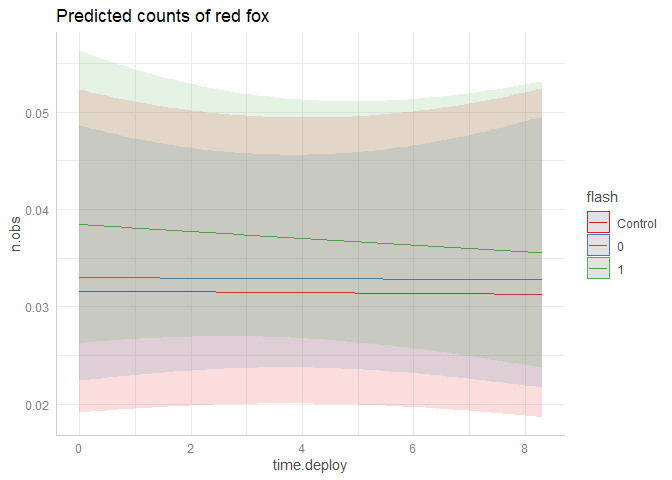
\includegraphics[width=.8\linewidth]{../R/glmm_sp_files/figure-gfm/rev-report-1.png}
		  \caption{Red fox}
		  	\label{fig:glmm_rev}
	\end{subfigure}
		\begin{subfigure}{.5\textwidth}
		  \centering
		  	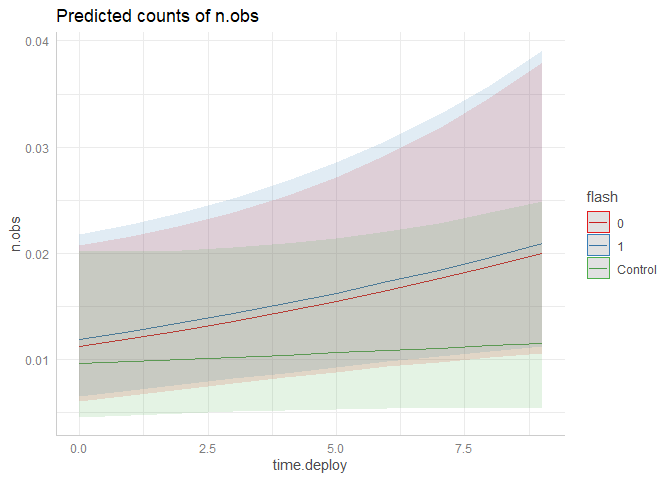
\includegraphics[width=.8\linewidth]{../R/glmm_sp_files/figure-gfm/grevling-report-1.png}
		  \caption{Badger}
		  	\label{fig:glmm_grvl}
	\end{subfigure}
		\begin{subfigure}{.5\textwidth}
		  \centering
		  	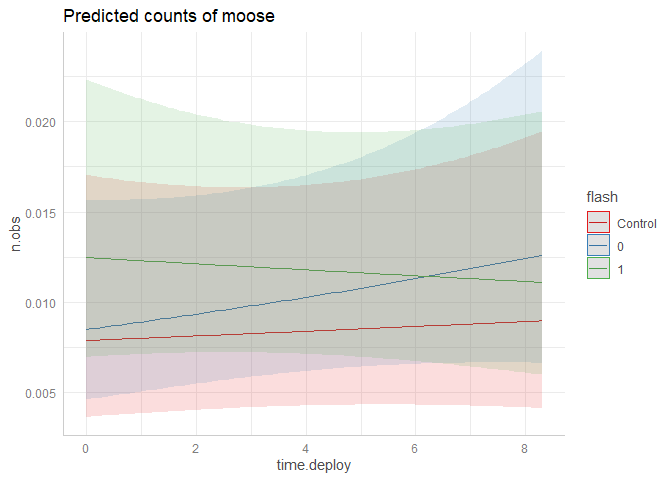
\includegraphics[width=.8\linewidth]{../R/glmm_sp_files/figure-gfm/elg-report-1.png}
		  \caption{Moose}
		  	\label{fig:glmm_elg}
	\end{subfigure}
		\begin{subfigure}{.5\textwidth}
		  \centering
		  	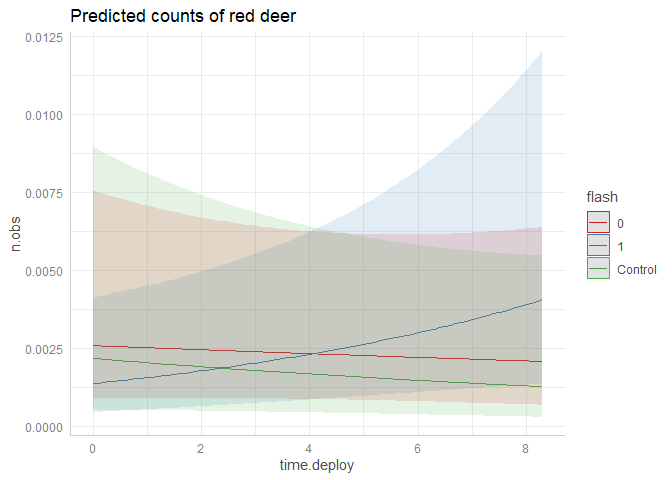
\includegraphics[width=.8\linewidth]{../R/glmm_sp_files/figure-gfm/hjort-report-1.png}
		  \caption{Red deer}
		  	\label{fig:glmm_hjort}
	\end{subfigure}
		\begin{subfigure}{.5\textwidth}
		  \centering
		  	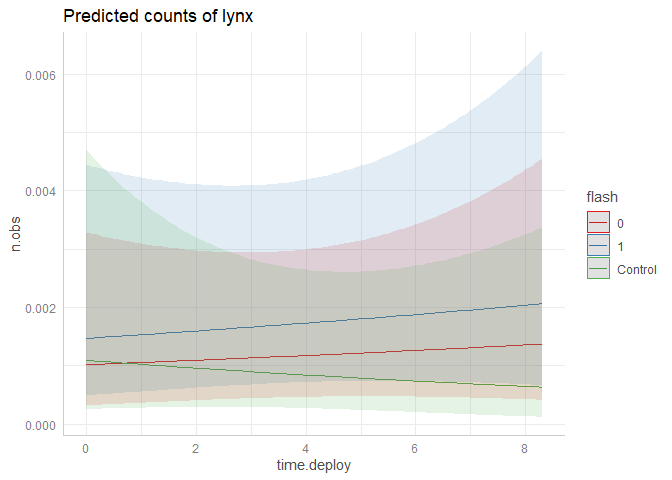
\includegraphics[width=.8\linewidth]{../R/glmm_sp_files/figure-gfm/gaupe-report-1.png}
		  \caption{Lynx}
		  	\label{fig:glmm_gaup}
	\end{subfigure}
		\caption{Fitted GLMM model to each species}
	\label{fig:glmm_sp}
\end{figure}



\begin{figure}
		\begin{subfigure}{.4\textwidth}
		  \centering
	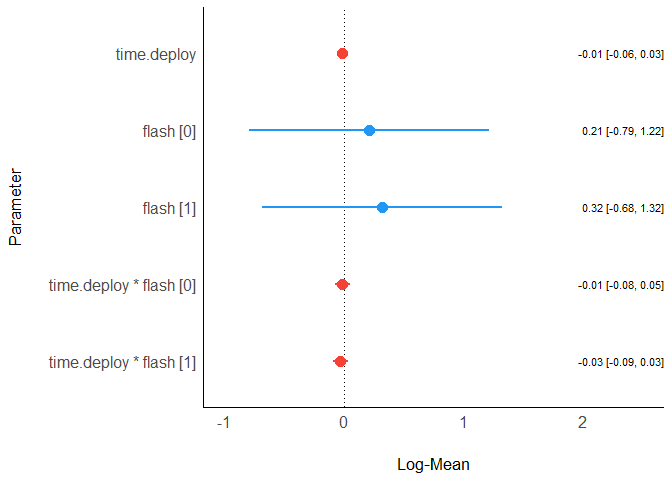
\includegraphics[scale=.4]{../R/glmm_sp_files/figure-gfm/parameters-1.png}
\caption{Intercept included}
		\label{fig:para_raa1}
	\end{subfigure}
		\begin{subfigure}{.4\textwidth}
		  \centering
	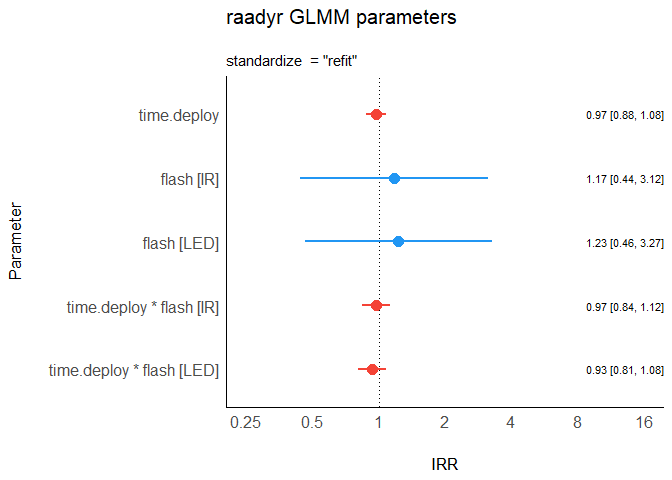
\includegraphics[scale=.4]{../R/glmm_sp_files/figure-gfm/parameters-2.png}
\caption{with values printed}
		\label{fig:para_raa2}
	\end{subfigure}
		\begin{subfigure}{.8\textwidth}
		  \centering
	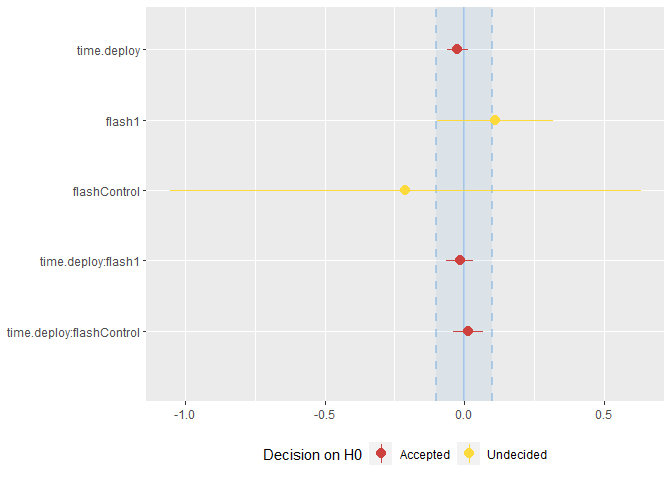
\includegraphics[scale=1]{../R/glmm_sp_files/figure-gfm/parameters-3.png}
\caption{Equivalence test}
		\label{fig:para_raa3}
	\end{subfigure}
		\caption{Visualising model parameters}
	\label{fig:para_sp}
\end{figure}




\clearpage %to force the insertion of parameters table
\pagestyle{fancy}

\section{Roe deer}
Roe deer was the most common species detected by the CTs, with a total number of 1709 events.
The species was detected at all times of day, with marked peaks of activity during the twilight hours.
Looking at the density curves in figure \ref{fig:raadyr}c, the overall activity pattern was consistent between the three types of periods (control, IR and white LED). 
The detection rates were also similar, as demonstrated in figure \ref{fig:raadyr}a.

The GLMM explaining variation in detection rate had a substantial explanatory power (conditional R2 = 0.45), but the part related to the fixed effects alone (marginal R2) was just 0.002.
In other words, most of the explained variation in detection rate was due to seasonal changes and variation between the different camera sites captured in the random terms.
In a standard null hypothesis significance test (NHST) no parameters were significant.

The equivalence test in figure \ref{fig:raadyr}b accepted the validity of H0 (that there were no effect) for the effect along the time axis in all three types of periods.
However, the detection rate varied a lot in all periods, which hindered a decision on the main effect of IR and white LED periods. 


\begin{figure}
\centering
	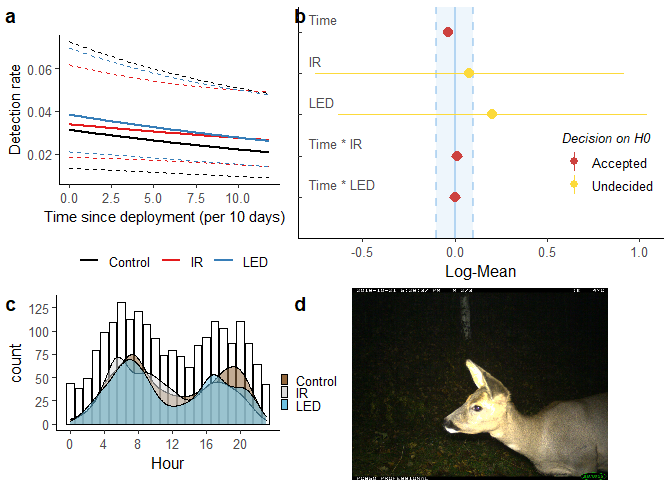
\includegraphics[scale=.9]{../R/glmm_sp_files/figure-html/parameters-1.png}
\caption[Roe deer]
{Roe deer %\par \small
 a) The predicted detection rate of roe deer for each level of the flash-variable. Confidence intervals (CI) represented by dotted lines.\\
b) Model parameters presented in an equivalence test. ROPE is set to $\pm$0.1 Log-Mean, $CI =1 - 2\times \alpha$.\\ 
c) Bars represent the raw count of total roe deer detections per hour of the day, and density curves show the overall pattern for each group.\\
d) LED-CT photograph of a roe deer. The deer passed the camera repeatedly and often stopped in front of the flashing light}\label{fig:raadyr}
\end{figure}


\newpage
\section{Red fox}

The red fox was the second most common species with 913 events.
The red fox was also active during the whole day, but with a more pronounced peak in the late evening continuing until the break of day, as visualised in figure \ref{fig:rev}c.
The overall pattern was similar between each group (Control, IR, white LED), and the overall effect of white LED was minor.

The GLMM explaining variation in detection rate of red fox had a substantial explanatory power (conditional R2 = 0.19), but the part related to the fixed effects alone (marginal R2) was just 0.001.
In other words, most of the explained variation in detection rate was due to seasonal changes and variation between the different camera sites captured in the random terms.
No parameters were significant in a standard NHST, and considering the equivalence test in figure \ref{fig:rev}b, the effect of time was practically equivalent for all types of periods.
However, the large variation in the main effect of  IR and white LED hinders any decision on H0. %, although the estimate of white LED (0.18) hints at an attractant effect. %IMRkomm: Men p-verdien er knallhøy, så jeg ville ikke klassifisert dette som et hint mot effekt.

\begin{figure}
		  \centering
	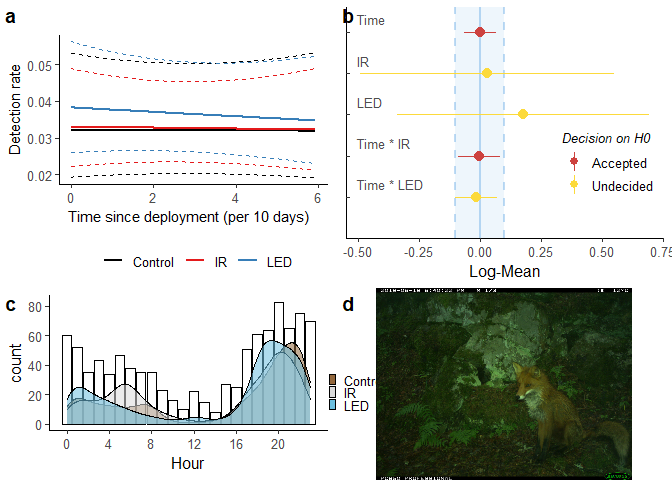
\includegraphics[scale=.9]{../R/glmm_sp_files/figure-html/rev2-1.png}
\caption[Red fox]
{Red fox %\par \small 
a) The predicted detection rate of red foxes for each level of the flash-variable. Confidence intervals (CI) represented by dotted lines.\\ 
b) Model parameters presented in an equivalence test. ROPE is set to $\pm$0.1 Log-Mean, $CI =1 - 2\times \alpha$.\\ 
c) Bars represent the raw count of total fox detections per hour of the day, and density curves show the overall pattern for each group.\\
d) LED-CT photograph of a red fox. The fox stopped in front of the flashing camera and waited for a following individual before they continued.}\label{fig:rev}
\end{figure}


\newpage
\section{Badger}


\begin{figure}
		  \centering
	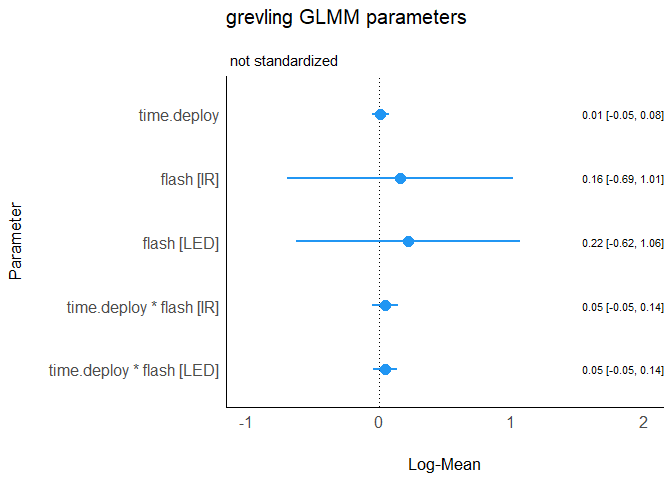
\includegraphics[scale=.9]{../R/glmm_sp_files/figure-html/grevling2-1.png}

\end{figure}

For badger, the model explaining variation in detection rate has a substantial explanatory power (conditional R2 = 0.42), but the part related to the fixed effects alone (marginal R2) is just 0.006. %AMkomm: her må det mer



%Sp:
%-Nth most common with n events,
%	-at n of the 56 sites 
%- activity pattern
%	-compared to expected activity from literature (cite)
%	-LED exposure (ie. activity during night
%	(-activity-density with and without event-filter?)
%-The model
%	-TK parameter(s) was (non-|significant) in SNHT (see table \ref{tab:param})
%	-Equivalence test says (mention 2nd gen p-value)
%	-ggeffects plot shows...
%-Conclusive sentence on species






\newpage
\section{Hare}


\begin{figure}
		  \centering
	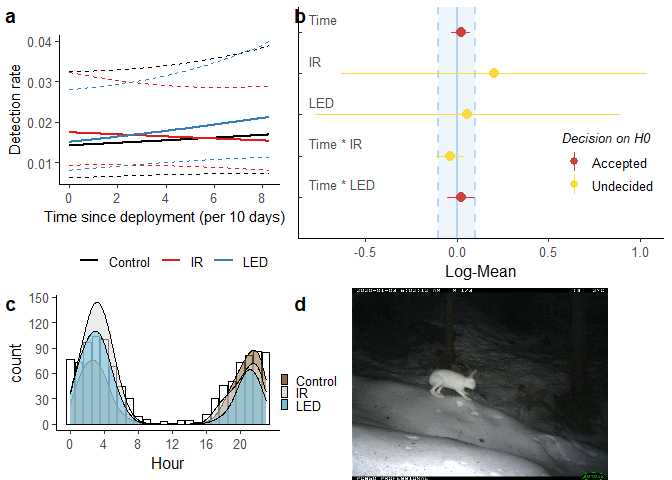
\includegraphics[scale=.9]{../R/glmm_sp_files/figure-html/hare2-1.png}

\end{figure}





\newpage
\section{Red squirrel}

\begin{figure}
		  \centering
	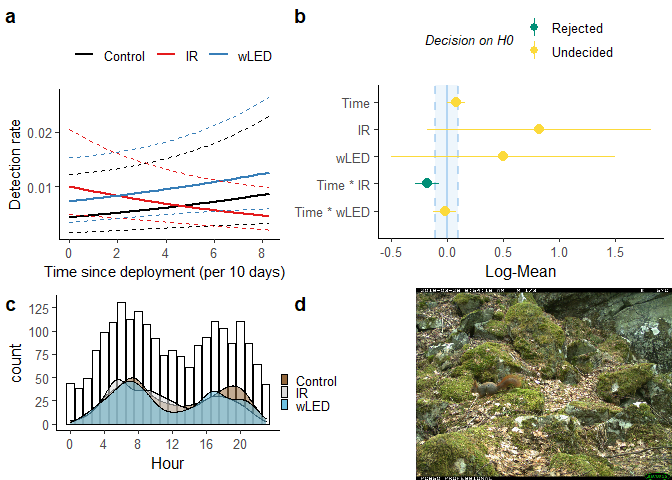
\includegraphics[scale=.9]{../R/glmm_sp_files/figure-html/ekorn2-1.png}

\end{figure}







\newpage
\section{Moose}

\begin{figure}
		  \centering
	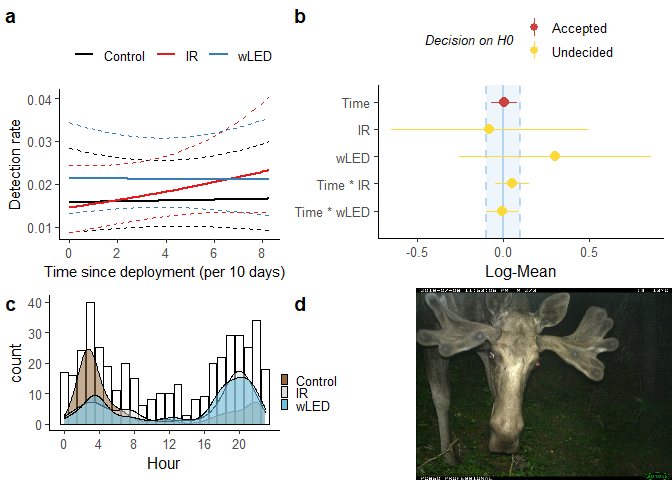
\includegraphics[scale=.9]{../R/glmm_sp_files/figure-html/elg2-1.png}

\end{figure}




\newpage
\section{Red deer}

\begin{figure}
		  \centering
	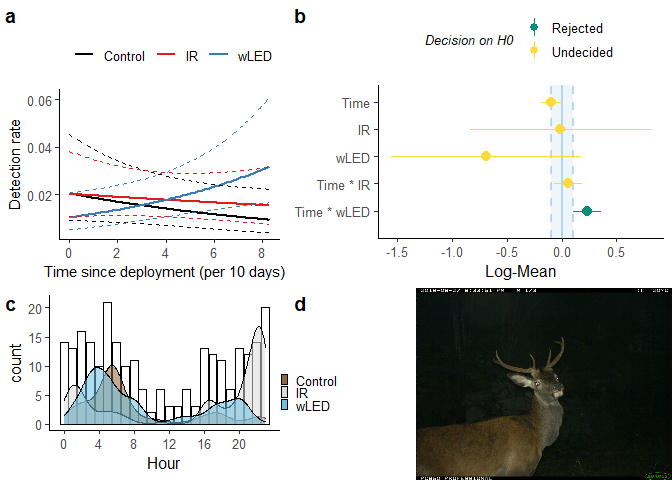
\includegraphics[scale=.9]{../R/glmm_sp_files/figure-html/hjort2-1.png}
\caption[Red deer]
{Red deer}
\end{figure}






\newpage
\section{Pine marten}

\begin{figure}
		  \centering
	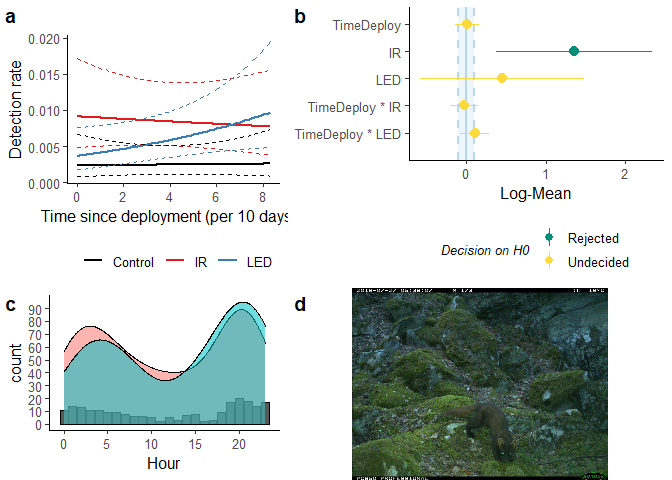
\includegraphics[scale=.9]{../R/glmm_sp_files/figure-html/maar2-1.png}
\caption[Pine marten]
{Pine marten}
\end{figure}






\newpage
\section{Lynx}


\begin{figure}
		  \centering
	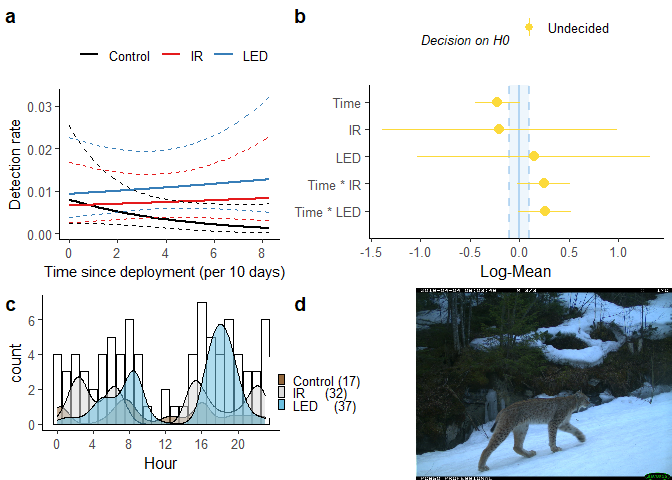
\includegraphics[scale=.9]{../R/glmm_sp_files/figure-html/gaupe2-1.png}
\caption[Lynx]
{Lynx}
\end{figure}


